%%% fs-seim-experiments - Experiments

\label {fs-experiments}

In order to estimate the performance, we implemented a prototype based on the proposed approach. As a stream processing task, we apply the computation of inverted index for 1000 Wikipedia documents. The logical pipeline of this computation is shown in Figure ~\ref{inverted-index}. First map operation accepts Wikipedia documents and outputs pairs of words and corresponding positions. The next part of the pipeline accepts pairs of word and positions and computes updated index and the actual changelog. 

This stateful transformation is implemented in the form of groping and map operation with a cycle, as it was shown in the previous section. Regarding the physical deployment, the full logical graph is deployed on each computational unit or worker. Documents are randomly shuffled before the first map operation. Word positions are partitioned by word before grouping. The other links are implemented as simple chain calls.

\begin{figure}[htbp]
  \centering
  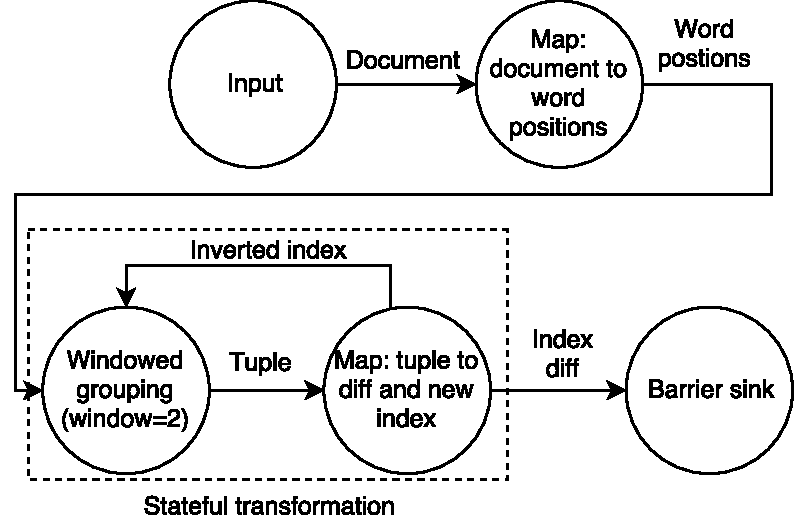
\includegraphics[width=0.48\textwidth]{pics/inverted-index}
  \caption{Logical pipeline for inverted index}
  \label {inverted-index}
\end{figure}

Our experiments were performed on clusters of 2, 4, 6, 8, and 10 nodes. Each node is an AWS EC2 micro instance with 1GB RAM and 1 core CPU.

As a key metric in our experiment, we take the ratio of arrived at the barrier items count to the number of the valid items among them. This value clearly represents the overhead of our approach. 

The relation between the number of workers, the delay between input documents and the proposed ratio is shown in Figure ~\ref{experiment}. As expected, the peak of the ratio is achieved when the delay between documents is short (less than 50 ms). This behavior can be explained by the fact that a few workers cannot effectively deal with such intensive load. Nevertheless, the proportion of invalid items reduces down to 1.3 with the increase of workers number within fixed high input rate. The reason behind this fact is the decrease of load on each specific node. Under non-extreme load, the ratio is under 1.1 for all considered number of workers. These results confirm that the ratio does not increase with the growth of the number of nodes.

Therefore, the most important conclusion of the experiments is that proposed method is scalable. Additionally, it is shown that the ratio of all items to the valid items is quite low for multiple workers even when the input rate is very high.

\begin{figure}[htbp]
  \centering
  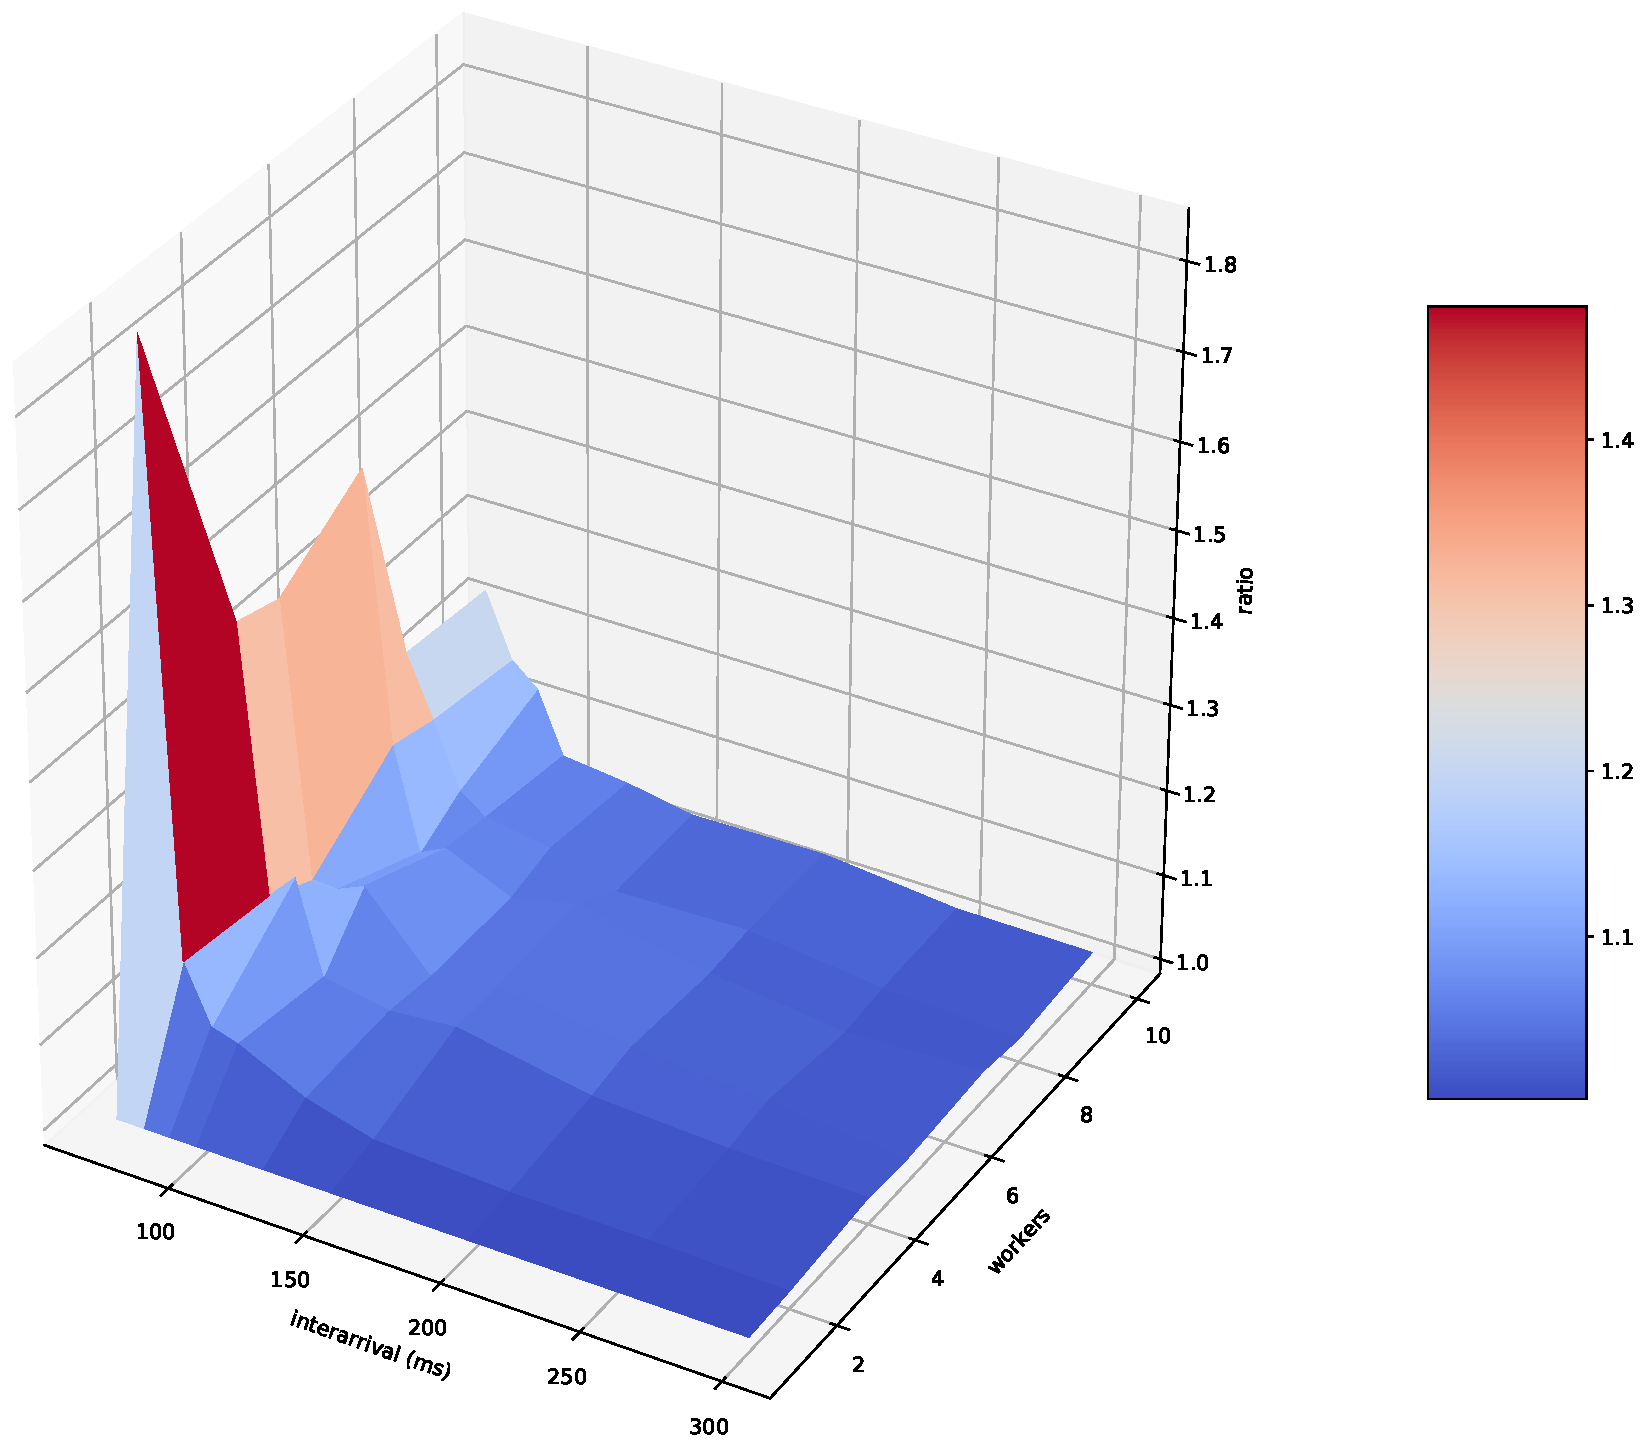
\includegraphics[width=0.48\textwidth]{pics/experiment}
  \caption{Experiment results}
  \label {experiment}
\end{figure}
